\documentclass{sig-alternate}

\usepackage{multirow}
\usepackage{graphics}
\graphicspath{ {figures/} }

\begin{document}

\conferenceinfo{WWW}{'15 Florence, Italy}


\title{Observing The State of Linked Open Data Cloud Metadata}

\numberofauthors{1}
\author{\alignauthor $\dagger\ddagger$ Ahmad Assaf, $\ddagger$ Aline Senart, and $\dagger$ Rapha\"{e}l Troncy \\
\affaddr$\dagger${EURECOM, Sophia Antipolis, France} \\ \affaddr$\ddagger${ SAP Labs, Sophia Antipolis, France} \\
\email{$\dagger$firstName.lastName@eurecom.fr, $\ddagger$firstName.lastName@sap.com}
}

\maketitle

\keywords{Data Profiling, Metadata, Dataset Profile, LOD Cloud}

\section{Introduction}
From 12 datasets cataloged in 2007, the Linked Open Data (LOD) cloud\footnote{http://datahub.io/dataset?tags=lod} has grown to nearly 1000 datasets containing more than 82 billion triples \cite{BizerHeath2009}. Data is being published by both public and private sectors and covers a diverse set of domains from life sciences to media or government data. The Linked Open Data cloud is potentially a gold mine for organizations and individuals who are trying to leverage external data sources in order to produce more informed business decisions \cite{Boyd2011}. However, the heterogeneous nature of data sources reflects directly on the data quality as these sources often contain inconsistent as well as misinterpreted and incomplete metadata information. Considering the significant variation in size, the languages used and the freshness of the data, one realizes that finding useful datasets without prior knowledge is increasingly complicated.\\

We have created a tool\footnote{https://github.com/ahmadassaf/opendata-checker} that automatically validates, corrects and generates dataset metadata for CKAN based data portals. In this poster, we present the results of running it on the LOD cloud hosted on the DataHub and comparing the results with those of Africa's largest open data portal, openAfrica. The results demonstrate that the general state of LOD cloud needs more attention as most of the datasets suffer from bad quality metadata lacking some informative metrics needed to facilitate dataset search. The noisiest metadata values were access information such as licensing information, resource descriptions as well as resource reachability problems.

\section{Metadata Profiling}

Data portals expose a set of information about each dataset as metadata. The model used varies across portals. However, a standard model should contain information about the datasets title, description, maintainer email, update and creation date, etc. We divided the metadata information into the following:
\textbf{General information}: General information about the dataset. e.g. title, description, ID, etc. This general information is manually filled by the dataset owner. In addition to that, tags and group information is required for classification and enhancing dataset discoverability. This information can be entered manually or inferred modules plugged into the topical profiler.
\textbf{Access information}: Information about accessing and using the dataset. This includes the dataset URL, license information i.e. license title and URL and information about the datasets resources. Each resource has as well a set of attached metadata e.g. resource name, URL, format, size, etc.
\textbf{Ownership information}: Information about the ownership of the dataset. e.g. organization details, maintainer details, author, etc. The existence of this information is important to identify the authority on which the generated report and the newly corrected profile will be sent to.
\textbf{Provenance information}: Temporal and historical information on the dataset and its resources. For example, creation and update dates, version information, version, etc. Most of this information can be automatically filled and tracked.

\section{Experiment Details}
The results discussed below are based on the LOD cloud hosted on CKAN\footnote{http://ckan.org}. It contained 259 datasets at the time of writing this poster. For comparison, we have also profiled the openAfrica data portal\footnote{http://africaopendata.org/} containing 1653 datasets.\\
A CKAN dataset metadata describes three main sections in addition to the core datasets properties. Those are the groups, tags and resources. Each section contains a set of metadata corresponding to one or more metadata type. For example, a dataset resource will have general information such as the resource name, access information such as the resource url and provenance information such as creation date. Our tool generates a report aggregating all the problems in all these sections, fixing field values when possible. Errors can be the result of missing metadata fields, undefined field values or field value errors e.g. unreachable URL or incorrect email address.\\\\

\section{Results and Evaluation}

We discovered that the general state of the LOD datasets needs attention as most of them lack informative access information and their resources suffer low availability. These two metrics are of high importance for enterprises looking to integrate and use external linked data. We found out that the most erroneous information for the dataset core information were ownership related as 41\% were missing or undefined. Datasets resources have the poorest metadata. 64\% of the general metadata, all the access information and 80\% of the provenance information contained missing or undefined values. Figure \ref{fig:1} shows the percentage of errors found in metadata fields by section.

We notice that 42.85\% of the top metadata problems can be fixed automatically. 44.44\% of these problems can be fixed by our tool while the others need tools that are plugged into the data portal. We further present and discuss the results grouped by metadata information type below.

\begin{figure}[!hpt]
\centering
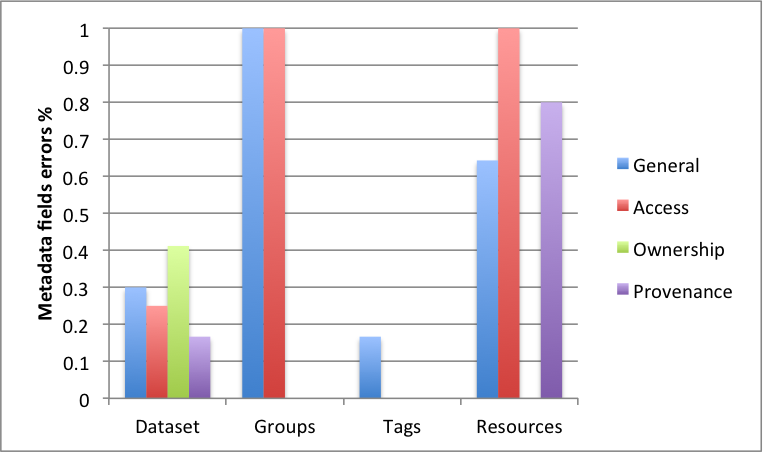
\includegraphics[width=.8\linewidth]{metadata_noise_by_section.png}
\caption{Error \% by section}
\label{fig:1}
\end{figure}

\textbf{General information} 34 datasets (13.13\%) did not have valid \texttt{notes} values. \texttt{tags} information for the datasets were complete except for the \texttt{vocabulary\_id} as it was missing from all the datasets' metadata. All the datasets \texttt{groups} information were missing \texttt{display\_name, description, title, image\_display\_url, id, name}.

\textbf{Access information} 25\% of the datasets access information (being the dataset URL and any URL defined in its groups) has issues related to them (missing or unreachable URLs).
Three datasets (1.15\%) did not have a URL defined while 45 datasets (17.3\%) defined URLs were not accessible at the time writing this poster.\\
On the datasets resources level, we noticed wrong or inconsistent values in the \texttt{size} and \texttt{mimetype} fields. 20 (1.87\%) resources had incorrect \texttt{mimetype} defined, while 52 (4.82\%) had incorrect \texttt{size} values. These values have been automatically fixed based on the values defined in the HTTP response header. However, 44 datasets have valid \texttt{size} field values and 54 have valid \texttt{mimetype} field values where they were not reachable, thus providing incorrect information.\\
15 (68\%) fields of all the other access metadata are missing or have undefined values. Looking closely, we noticed that most of these problems can be easily fixed automatically by tools that can be plugged to the data portal. However, the most important missing information which require manual entry are the dataset's \texttt{name} and \texttt{description} were missing from 817 (76.49\%) and 98 (9.17\%) resources respectively.
A total of 334 resources (31.27\%) URLs were not reachable, thus affecting highly the availability of these datasets. Their breakdown according to their type is: 211 (63.17\%) resources did not have valid \texttt{resource\_type}, 112 (33.53\%) were files, 8 (2.39\%) and one (0.029\%) metadata, example and documentation types.
The noisiest part of the access metadata was license information. A total of 43 datasets (16.6\%) did not have a defined \texttt{license\_title} and \texttt{license\_id} fields, where 141 (54.44\%) had missing \texttt{license\_url} field. However, we managed to normalize 123 (47.49\%) of the datasets' license information using the manual mapping file.

\textbf{Ownership information} Ownership information is divided into direct ownership (author and maintainer) and organization information. Four fields (66.66\%) of the direct ownership information were missing or undefined. The breakdown for the missing information is: 55.21\% \texttt{maintainer\_email}, 51.35\% \texttt{maintainer}, 15.06\% \texttt{author\_email}, 2.32\% \texttt{author}. Moreover, our tools performs checks to validate existing email values. 11 (0.05\%) and 6 (0.05\%) of the defined \texttt{author\_email} and \texttt{maintainer\_email} fields were not valid email addresses respectively.

\textbf{Provenance information} 80\% of the resources provenance information were missing or undefined. However, most of the provenance information e.g. \texttt{metadata\_created, metadata\_modified)} can be computed automatically by tools plugged into the data portal. The only field requiring manual entry is the \texttt{version} field which was found to be missing from 60.23\% of the datasets.

\begin{figure}[!hpt]
\centering
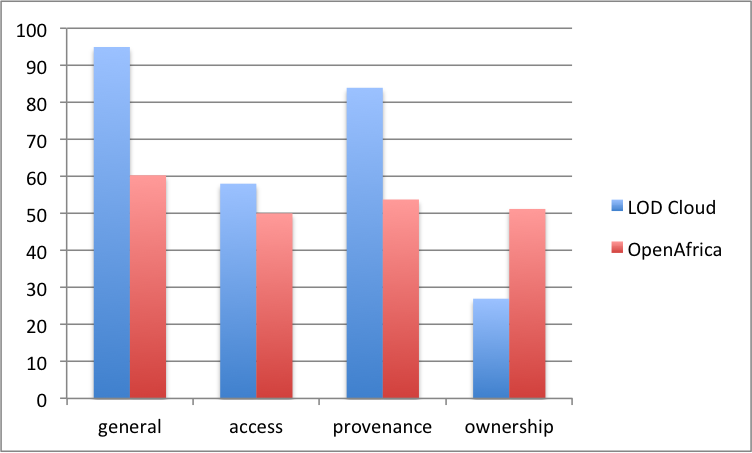
\includegraphics[width=.8\linewidth]{metadata_LOD_vs_Africa.png}
\caption{Average Error \% by section LOD vs. openAfrica}
\label{fig:2}
\end{figure}

Figure \ref{fig:2} shows the comparison between the average error rates in each metadata section in the LOD cloud and openAfrica. We notice that the quality of LOD cloud datasets is worse in the general, access and provenance sections. In the access information, the noted differences where in the percentage of unreachable URLs, \texttt{hash} and \texttt{size} fields. Moreover, provenance information had a clear gap as for example 86.8\% of the LOD cloud \texttt{version} information was missing while it was complete in all the openAfrica datasets. However, the LOD cloud had better ownership and license information where 82.03\% of the openAfrica datasets license information couldn't be normalized while it was only 52.5\% in the LOD cloud.
\bibliographystyle{abbrv}
\bibliography{www15-poster}

\end{document}
